\chapter{Implementation}
\label{chap:implementation}

This chapter discusses in detail all the implementation aspects of the framework, showing all its characterizing elements.
First, the reasons for choosing Kotlin as the language to implement the framework are explained.
Then, for each module, the logic governing it, the main classes, and usage scenarios will be analyzed.
Finally, the chapter will conclude with a discussion of the configuration DSL and the platform DSL.

\section{Languages with multiplatform targets}
\label{sec:languages-multiplatform-targets}

Pulverization is born in a context where device heterogeneity, understood as the strong difference in computational terms of devices as well as
diversity of architectures, is the norm.
For those reasons, we can deal with networks of embedded devices (which have very limited computational resources) up to networks of computers with
high computational power and memory.
Nowadays, architectures that combine these two scenarios are increasingly common, thus having to manage architecturally heterogeneous networks of
devices.

For these reasons, it is necessary to build a framework that can support as many architectures and platforms as possible to maximize the number
of devices on which the pulverized system can run.

In this context, the choice of the language to implement the framework is crucial.
A cross-platform language (or even known as multiplatform language) is a language that allows the same code to be compiled for different platforms.
The trend over the last years is to use the same language to span over several runtime and VMs (e.g. JVM, JavaScript, native platforms, etc.) in order
to reduce the effort of maintaining the codebase and to increase the portability of the application.
The other main advantage of using a multiplatform language is that all the shared concepts and logic can be implemented in a single codebase that
can be reused in all the specific platforms.

In this way, we can use one programming language and manage the targeting of multiple platforms effectively (see~\Cref{fig:mulitplatform-languages}).

\begin{figure}
	\centering
	\missingfigure[figwidth=\textwidth]{Show from an architectural perspective how a multiplatform language works}
	\caption{Diagram showing the philosophy of multiplatform languages.}
	\label{fig:mulitplatform-languages}
\end{figure}

\todo{Aggiungere paragrafo in cui si da un idea piu tecnica di come viene gestito il multiplatform. Ad esempio spiegando IR ecc.}

The two following sections will examine two of the main relevant language based on the JVM ecosystem that supports multiplatform targets.

\subsection{Scala Language}
\label{sec:scala-language}

The Scala programming language is a general-purpose programming language that is designed to combine object-oriented and functional programming in one
concise, high-level language.

Although Scala was born under the JVM, it has been extended to support other platforms such as JavaScript, and native platforms.

Support for cross-platform is enabled through external plugins and not directly by the Scala compiler itself.
The plugin enables compiler extensions allowing the generation of \emph{intermediate representations} (IRs) containing platform-specific aspects;
with the IR, the compiler makes optimization, linking and other dependencies management.

The~\Cref{lst:scala-cross-platform} shows the minimal configuration required to enable the cross-platform support for the Scala language,
in particular are enabled JVM, JavaScript and native platforms.

\lstinputlisting[
	float,
	language=scala,
	caption={Minimal configuration to enable cross-platform support for Scala.},
	label={lst:scala-cross-platform}
]{listings/scala-cross-platform.sbt}

\begin{figure}
	\centering
	\begin{subfigure}{.45\textwidth}
		\centering
		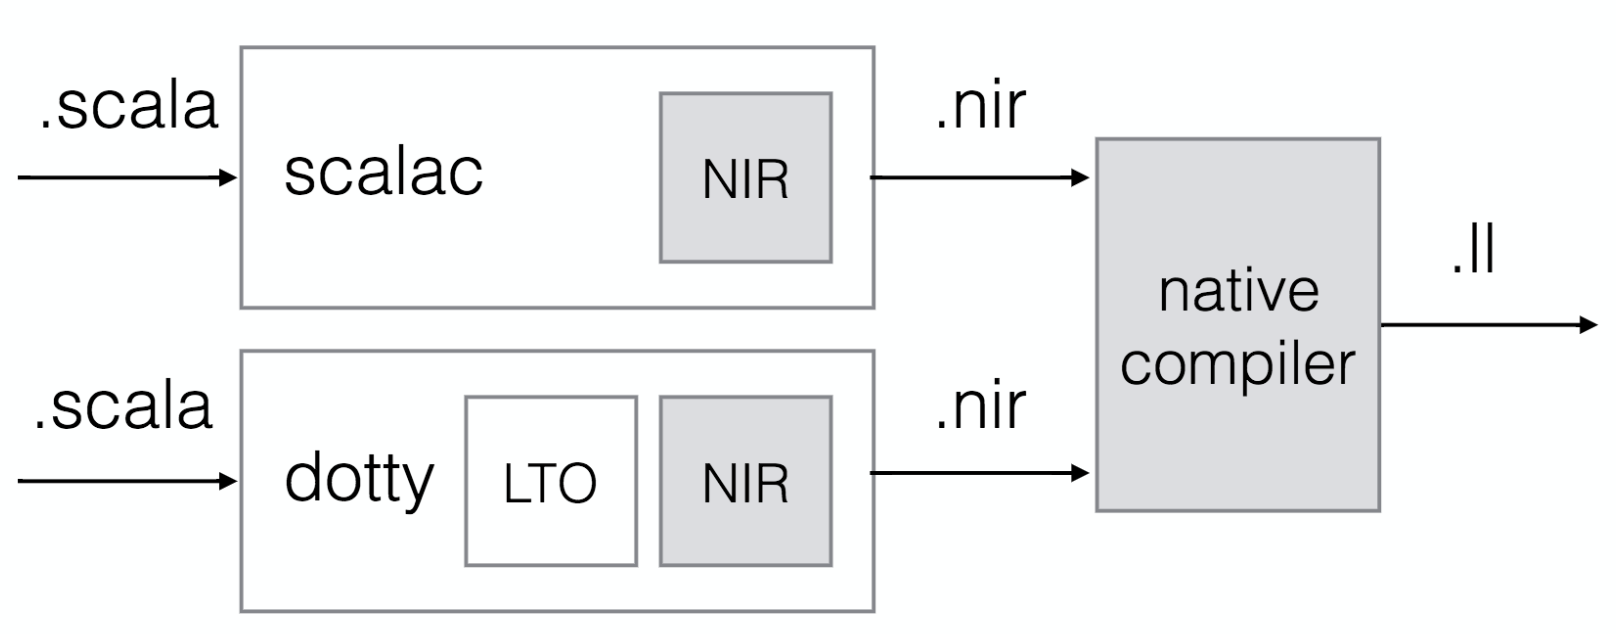
\includegraphics[width=0.95\linewidth]{figures/scala-native-ir.png}
		\caption{Scala native compilation pipeline.}
		\label{fig:scala-native-ir}
	\end{subfigure}
	\begin{subfigure}{.45\textwidth}
		\centering
		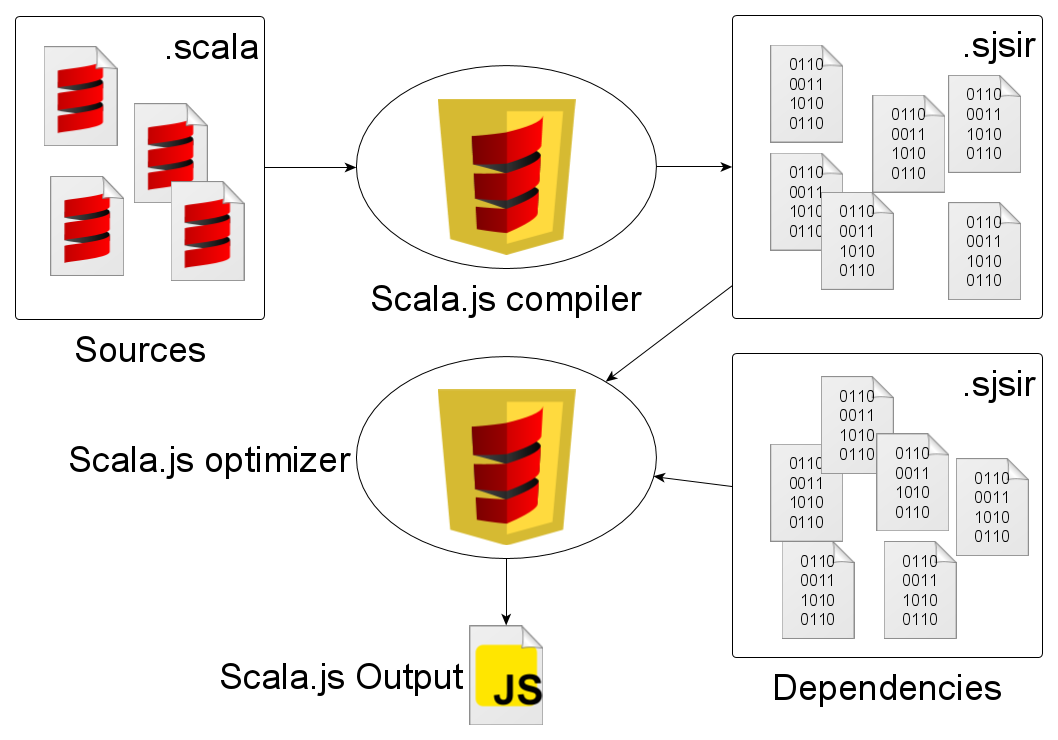
\includegraphics[width=.95\linewidth]{figures/compilation-pipeline.png}
		\caption{Scala.js compilation pipeline.}
		\label{fig:scala-js-ir}
	\end{subfigure}
	\caption{Representation of the Scala Native and Scala.js IR generation and compilation pipelines.}
	\label{fig:scala-ir}
\end{figure}

The~\Cref{fig:scala-ir} depicts the two main targets and for each one shows the compilation pipeline in particular, the~\Cref{fig:scala-native-ir}
shows the compilation pipeline for the native target, while the~\Cref{fig:scala-js-ir} shows the compilation pipeline for the JavaScript target.

For what concern the native target, the compilation pipeline is composed of the following steps~\cite{scala-native}:
\begin{itemize}
	\item \textbf{Scala code compiled into Native Intermediate Representation:} the \texttt{nscplugin} takes the Scala source code and inspecting the
	      AST, it generates the \texttt{.nir} files.
	\item \textbf{LLVM final compilation:} all the \texttt{.nir} files are compiled into \texttt{.ll} files and passed to the LLVM compiler that
	      produces the native binary file.
\end{itemize}

\todo{espandere la parte relativa a scala native}

The pipeline for the JavaScript target is quite more articulated but for the sake of simplicity, are reported only the main phases of the compilation
steps~\cite{Doeraene:256862}:
\begin{itemize}
	\item \textbf{Generation of the Scala.js IR:} the \texttt{scalajs-compiler} takes the Scala source code and generates the \texttt{.sjsir} files.
	\item \textbf{Optimization (linking):} in this phase the \texttt{scalajs-optimizer} takes the \texttt{.sjsir} files and performs optimizations
	      taking also other \texttt{.sjsir} files coming from dependencies.
	\item \textbf{Output file:} the \texttt{scalajs-optimizer} generates the \texttt{.js} file that is the output of the compilation.
\end{itemize}

During the first step, the \texttt{.scala} source files are compiled with scalac, augmented with the Scala.js compiler plugin.
The compiler plugin, comparatively to the rest of scalac, is small: it takes the internal compiler ASTs that have been lowered to contain JVM-style
classes, interfaces, methods and instructions, and turns them into Scala.js IR (\texttt{.sjsir} files).

The \texttt{.sjsir} files are similar to \texttt{.class} files, although they are AST-based (instead of stack-machine-based) and contain features
dedicated to JavaScript interoperability. The \texttt{.sjsir} format and specification are independent of Scala: which means that the linker is
independent of the language version.

\subsubsection*{Scala multiplatform ecosystem}

This section will examine the current ecosystem concerning the multiplatform support for the Scala language to have more awareness about the
usability of this technology.
In particular, will be addressed two main factors: the number of libraries that supports multiplatform targeting and the maturity of each platform.

At first glance, there is a strong sense of fragmentation of projects and various communities. Some communities pervasively support all three
platforms (JVM, JS, and native) while others do not, and this is reflected in the amount of multi-targeting compatible libraries.
For example, the \emph{typelevel} ecosystem supports all three platforms for all their main libraries:
\textbf{Cats Effects}~\footnote{\url{https://typelevel.org/cats-effect/}} and \textbf{FS2}~\footnote{\url{https://fs2.io/}}.
From the other side, the \emph{zio}~\footnote{\url{https://zio.dev/}} ecosystem supports only JVM and JavaScript while the native platform is an
experimental stage.
Even if the actual number of libraries is not so high, the Scala ecosystem is quite mature to be used in its multiplatform version.
Moreover, there is a lot of work being done by the Scala community to improve the multiplatform support for the language, so it's very likely that in
the future the number of libraries targeting multiplatform will increase.

To complete the analysis and to have a more complete picture of the Scala multiplatform ecosystem, will be examined the maturity of each platform.
Starting from \emph{Scala.js}, the platform is quite mature and stable: the project was born several years ago and it's used in production by many
companies, year to year several improvements were made to reach a high level of performance and stability~\cite{scala-js-performance, marr2016cross}.

Finally, the \emph{Scala Native} platform works quite well but has some limitations that make it not suitable for all production use.
One of the biggest and most important limitations is the lack of support for multithreading~\cite{scala-native-multithreading}.
If for some projects this limitation is not a problem, for others it can be a big issue; nevertheless, the \emph{typelevel} community dealt with this
restriction by implementing an event-loop-based concurrency model~\cite{scala-native-multithreading} to support the native projects.
Another limitation is represented by the supported architectures: at the time of writing, only the platforms supported by \emph{LLVM} can be targeted,
which means that not all the embedded devices can be supported.

\subsection{Kotlin Language}
\label{sec:kotlin-language}

Kotlin is a cross-platform, statically typed, general-purpose high-level programming language.
It's designed to interoperate fully with Java but also compile to JavaScript or native code via LLVM.

For what concern the multiplatform support of the language, Kotlin multiplatform is designed to simplify the development of cross-platform projects
by reducing the time spent writing and maintaining the same code for different platforms.

The Kotlin multiplatform use cases can be synthesized in the following points:
\begin{itemize}
	\item \textbf{Android and iOS applications} sharing the code between mobile platforms enable the building of cross-platform mobile applications
	      sharing the common code between Android and iOS.
	\item \textbf{Full-stack web applications} when building web applications, it's possible to share the code between the client and the server
	      reusing the same logic on both sides.
	\item \textbf{Multiplatform libraries} a multiplatform library with common code and its platform-specific implementations for JVM, JS, and Native platforms can be created. Once published, a multiplatform library can be used in other cross-platform projects as a dependency.
\end{itemize}

\begin{figure}
	\centering
	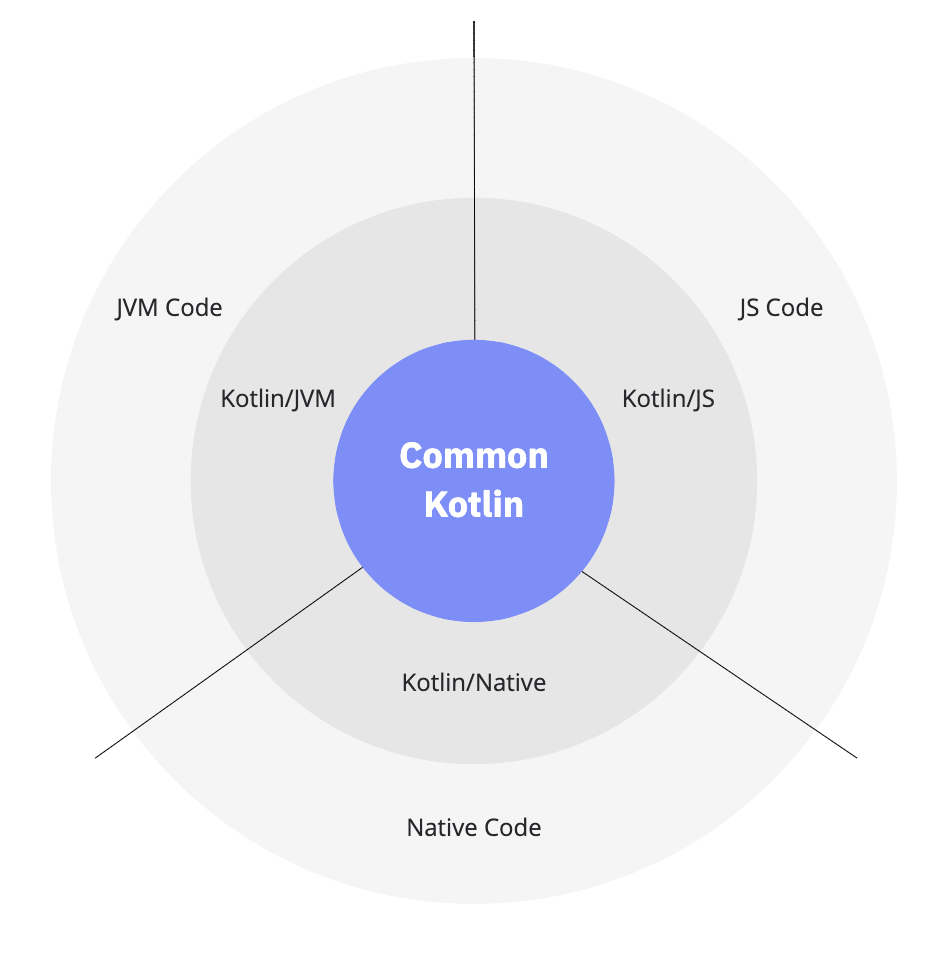
\includegraphics[width=.5\linewidth]{figures/kotlin-multiplatform.png}
	\caption{Kotlin multiplatform structure}
	\label{fig:kotlin-multiplatform-structure}
\end{figure}

The Kotlin multiplatform works using an onion-like structure (see~\Cref{fig:kotlin-multiplatform-structure}) where the common code is at the center
and works everywhere on all platforms; to interoperate with platforms, a specific version of Kotlin is used that includes platform-specific
libraries and tools. Through these platforms, you can access the platform's native code and leverage all native capabilities.

Similarly to Scala, the multiplatform support for Kotlin is enabled via a
Gradle~\footnote{\textbf{Gradle} is a build automation tool for multi-language software development. It's based on \emph{Apache Ant} and
	\emph{Apache Maven} introducing a Groovy and Kotlin DSL. The main supported languages are \emph{Java, Kotlin, Groovy} and \emph{Scala}.} plugin.
As for Scala, the plugin enables a series of tools and compiler extensions to support multiplatform development.

\lstinputlisting[
	language=kotlin,
	caption={},
	label={lst:koltin-multiplatform-setup}
]{listings/kotlin-multiplatform-setup.kts}

The~\Cref{lst:koltin-multiplatform-setup} shows a basic setup of Kotlin multiplatform using the Gradle plugin.

To share code between all the platforms, Kotlin provides a specific mechanism using a hierarchical structure of modules.
The common code is placed in the \texttt{commonMain} module and it's used to share the common business logic that applies to all the platforms.
Often there is the need to create several native targets that could potentially reuse a lot of the common logic and third-party APIs; Kotlin allows
to create a specific and flexible structure to reuse as much code as possible between the different targets.
The~\Cref{fig:kotlin-multiplatform-hierarchy} shows a possible representation of a Kotlin multiplatform project hierarchical structure.

\begin{figure}
	\centering
	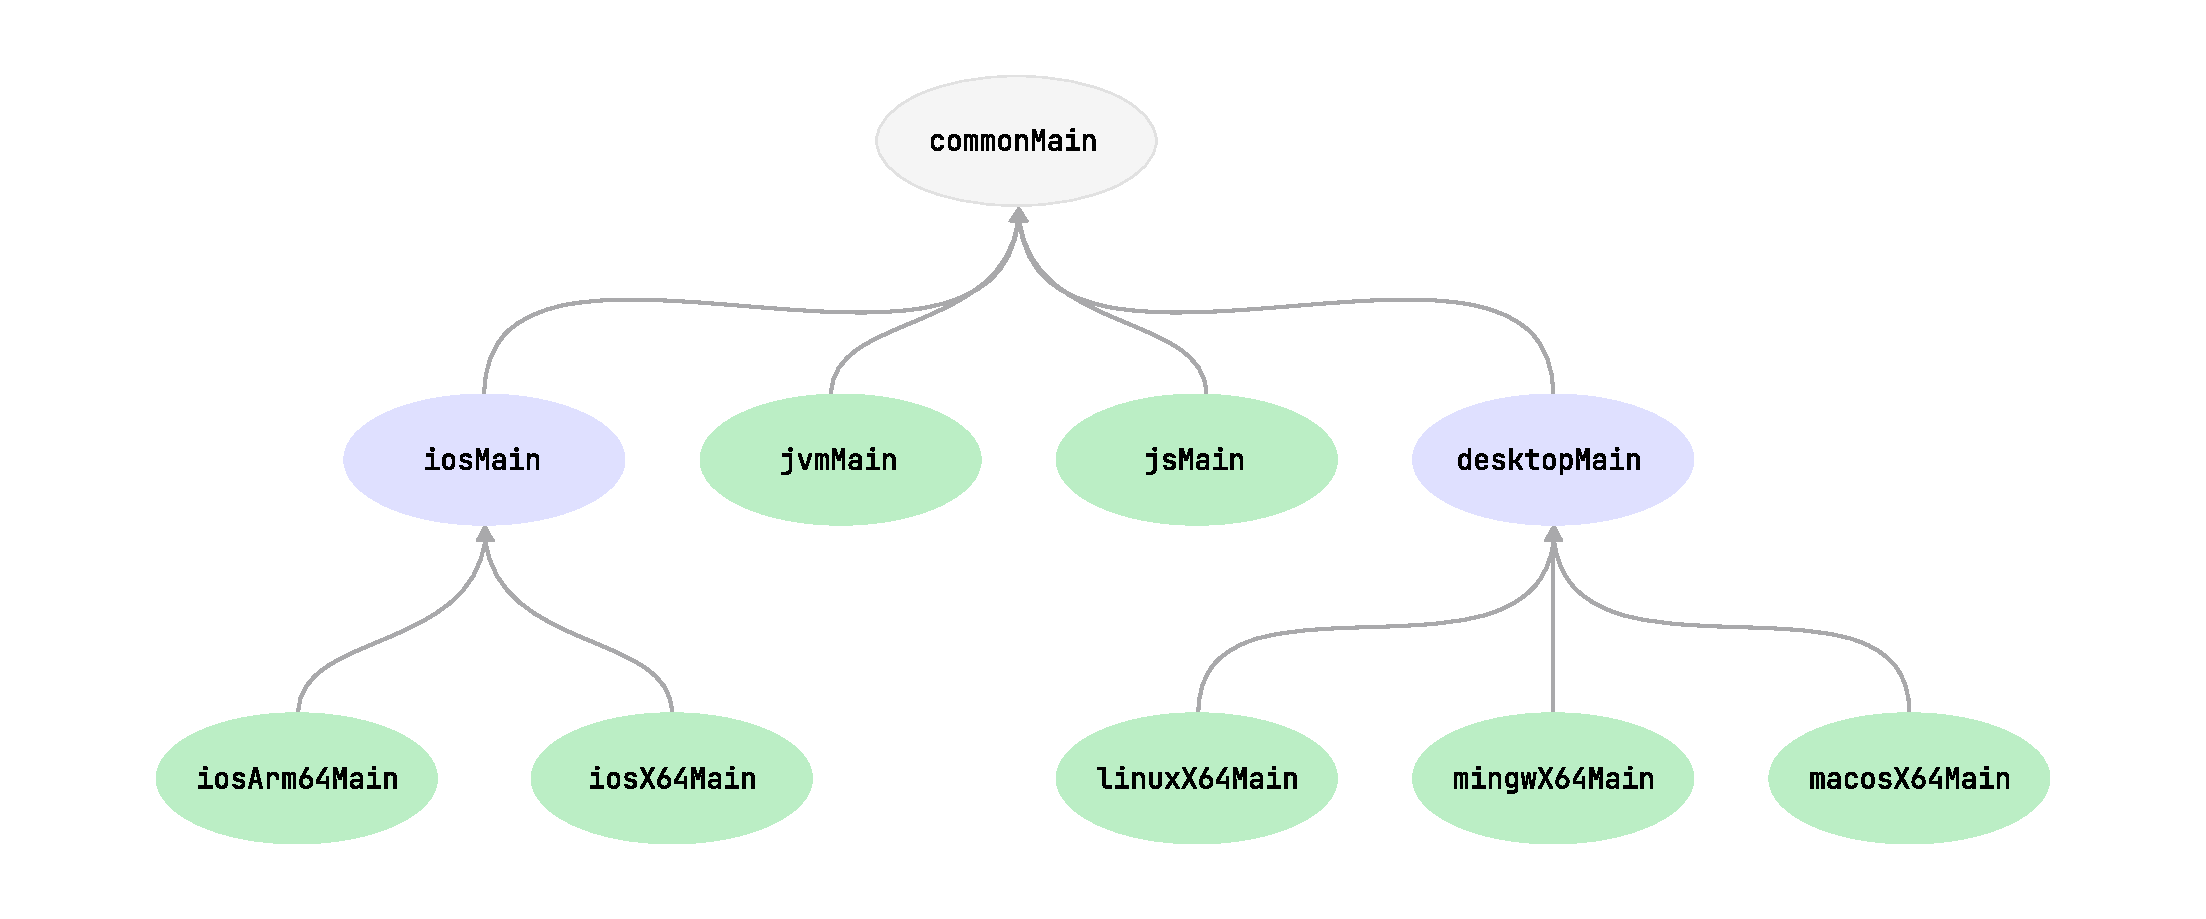
\includegraphics[width=\linewidth]{figures/kotlin-multiplatform-hierarchical-structure.pdf}
	\caption{Kotlin multiplatform hierarchical structure.}
	\label{fig:kotlin-multiplatform-hierarchy}
\end{figure}

To access the platform-specific APIs from the shared code, Kotlin provides a specific mechanism called \emph{expect/actual}
declarations~\footnote{\url{https://kotlinlang.org/docs/multiplatform-connect-to-apis.html}}.
With this mechanism, a common source set defines an expected declaration, and platform source sets must provide the actual declaration that
corresponds to the expected declaration.

\begin{figure}
	\centering
	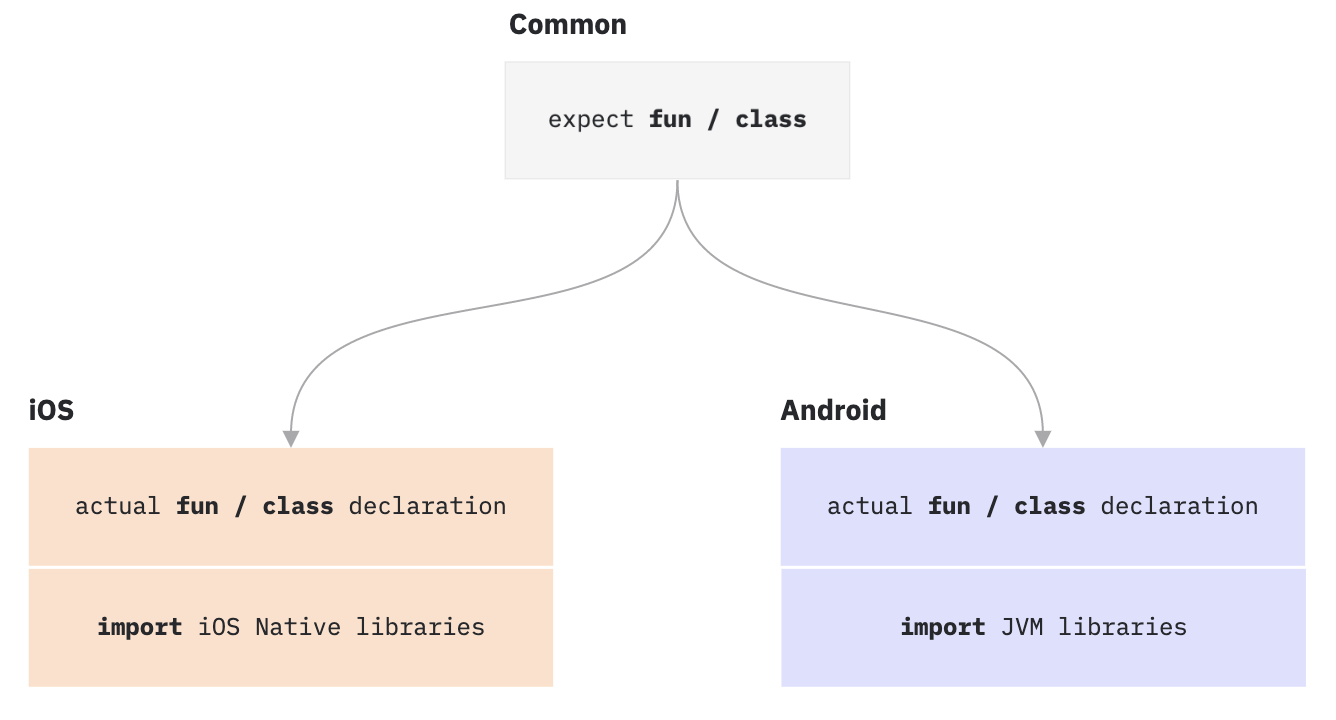
\includegraphics[width=\linewidth]{figures/expect-actual.png}
	\caption{Kotlin multiplatform expect/actual mechanism.}
	\label{fig:kotlin-multiplatform-expected-actual}
\end{figure}

The \emph{expect/actual} mechanism is shown in~\Cref{fig:kotlin-multiplatform-expected-actual} where a class in the common source set is marked as
\texttt{expect} and the platform-specific source set provides the actual implementation of the class.

The compiler ensures that every declaration marked as \texttt{expect} has a corresponding declaration marked as \texttt{actual} in the corresponding
platform modules. In this way, is guaranteed that every platform has an implementation for that class or function.

The following will be a brief introduction to how Kotlin can generate native code and js code from the same code base.

The \emph{Kotlin/JS IR} compiler is responsible for compiling Kotlin code into JavaScript code. The compiler backend rather than generating directly
JavaScript code generates an intermediate representation (IR) of the code which is subsequently compiled into JavaScript code.
This strategy enables aggressive optimizations, improving, for example, the generated code size.

The \emph{Kotlin/Native} compiler is responsible for compiling Kotlin code into native code. The compiler is available for all the main operating
systems (macOS, Linux, and Windows) and supports different targets like \textbf{iOS, Windows, macOS, Linux, Raspberry PI, STM32,} and
\textbf{WebAssembly}. Unfortunately, there aren't details about how the compiler pipeline works, but it's possible to see that the compiler generates
an IR representation of the code and then compiles it into native code via LLVM.
A relevant feature of \emph{Kotlin/Native} is the interoperability with \emph{C} code. This feature allows using existing C libraries in Kotlin using
the \emph{cinterop} tools that generate Kotlin bindings for the C library. The \emph{cinterop} tool requires a \texttt{.def} file that describes what
to include into bindings, in particular, are specified the \texttt{.a/.so} libraries to include and the \texttt{.h} files to parse. Finally, the
\emph{cinterop} tool generates a Kotlin library that can be used in the Kotlin code.

When a \emph{Kotlin/Native} library is distributed, a special file with extension \texttt{.klib} is generated. This file contains all the information and file specifics for each platform. It's a \texttt{.zip} file containing a predefined directory structure; for example,
the \texttt{foo.klib} when unpacked as \texttt{foo/} directory contains the following files and directories:
\begin{itemize}
	\item in a folder with the \emph{component name} is contained the serialized Kotlin IR
	\item in a folder \texttt{targets} are placed the platform-specific files, in particular in the folder \texttt{kotlin} there is Kotlin compiled
	      into LLVM bitcode; in the \texttt{native} folder there are the bitcode files of additional native objects
	\item the \texttt{linkdata} folder contains a set of \emph{ProtoBuf}~\footnote{Protocol Buffers (Protobuf) is a free and open-source
		      cross-platform data format used to serialize structured data.} files with serialized linkage metadata
	\item the \texttt{resources} folder contains resources such as images, fonts, and other files
	\item a \texttt{manifest} file in the java property format describing the library.
\end{itemize}

This structure allows to have a single \texttt{.klib} file that can be used in different platforms without the need to recompile the library for each
one of them.

\subsubsection*{Kotlin multiplatform ecosystem}

As already done for Scala, the ecosystem will be examined for Kotlin to get a better awareness of the usability of this technology.
Again, the number of supported libraries and the maturity of the framework will be considered.

Differently from the Scala multiplatform ecosystem, the Kotlin one seems to be more coherent and structured: lots of libraries
like \textbf{kotlinx.serialization}, \textbf{kotlinx.coroutines}, and \textbf{ktor} are available for all the target platforms supported by Kotlin.
The other difference is that most of the libraries are developed directly (or with the support of) the Kotlin team, this means that support and the
development is more aligned and coherent with the language itself.
The identification of the magnitude of libraries targeting Kotlin multiplatform is quite simple since a
site~\footnote{\url{https://libs.kmp.icerock.dev/}} collects all the available Kotlin multiplatform libraries. From this site can be seen that more
than 140 libraries are available for Kotlin multiplatform, spacing from different categories and applications. Of course, not all the available
libraries are collected on this site, but it's a good starting point to get an idea of the ecosystem.

For concern the maturity of the framework, the Kotlin multiplatform is still in beta, nevertheless, its stability and usability make it a
good candidate for a production-ready product. The Kotlin team is working hard to improve the framework and make it more stable and usable.
If in Scala the specific module for each supported platform (JS and native) is developed by an external community, reducing the guarantee of stability
and coherence with the language, in Kotlin the multiplatform module is developed by the JetBrains team itself, increasing the guarantee of stability
of the entire framework.

% - New section ---------------------------------------------------------------

\section{Core module}
\label{sec:core-module-impl}

% - New section ---------------------------------------------------------------

\section{Platform module}
\label{sec:platform-module-impl}

% - New section ---------------------------------------------------------------

\section{RabbitMQ module}
\label{sec:rabbitmq-module-impl}

% - New section ---------------------------------------------------------------

\section{Configuration DSL}
\label{sec:configuration-dsl-impl}

% - New section ---------------------------------------------------------------

\section{Platform DSL}
\label{sec:platform-dsl-impl}
